\documentclass[12pt]{article}
\usepackage{tikz}
\usepackage[utf8]{inputenc}
\pagestyle{empty}

\usetikzlibrary{arrows}

\tikzset{
  treeNode/.style = {align=center, inner sep=5pt, text centered},
  %black node
  nodeBlack/.style = {treeNode, circle, white, draw=black,
    fill=black, minimum width=25},
  %red node  
  nodeRed/.style = {treeNode, circle, red, draw=red, minimum width=25},
  %nil node  
  nodeNil/.style = {treeNode, circle, draw=black, minimum width=25}
}

\begin{document}
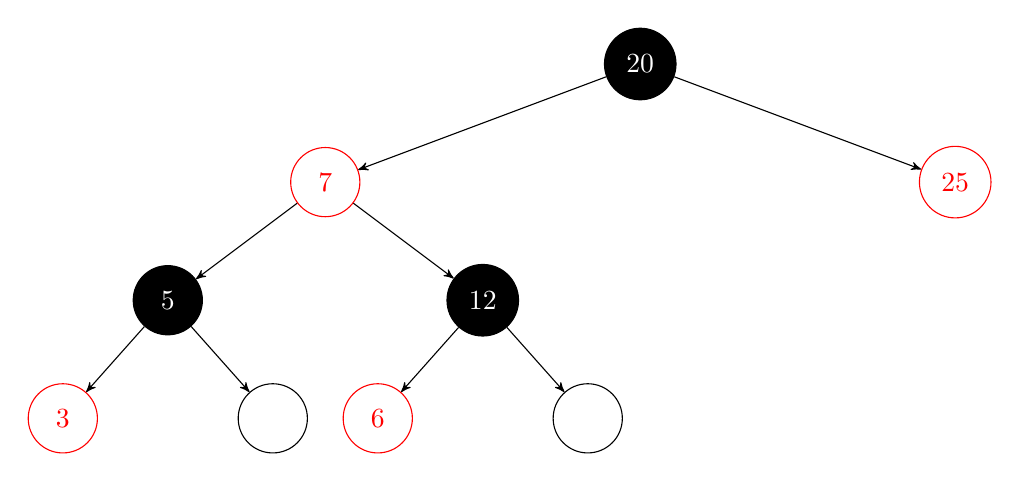
\begin{tikzpicture}[->,>=stealth',level/.style={sibling distance = 8cm/#1,
  level distance = 1.5cm}] 
\node [nodeBlack] {20}
    child{ node [nodeRed] {7} 
            child{ node [nodeBlack] {5} 
            	child{ node [nodeRed] {3} }
							child{ node [nodeNil] {}}
            }
            child{ node [nodeBlack] {12}
							child{ node [nodeRed] {6}}
							child{ node [nodeNil] {}}
            }                            
    }
    child{ node [nodeRed] {25}
		}
; 
\end{tikzpicture}
\end{document}
